\chapter{Wyniki eksperymentów: analiza procesu uczenia, interpretacja metryk i jakość heurystyk naprawczych}

W niniejszym rozdziale zaprezentowano wyniki eksperymentów porównawczych pomiędzy wariantem referencyjnym (\textit{Without Learning}, dalej w skrócie \textbf{NL}) a wariantem z włączonym potokiem ACE (\textit{With Learning}, dalej w skrócie \textbf{L}). Eksperymenty zostały przeprowadzone dla dwóch różnych modeli językowych: \textbf{GPT-5-nano} oraz \textbf{Minimax-2.5}. Oba warianty dla każdego modelu zostały uruchomione na tej samej, deterministycznej sekwencji 98 incydentów (epizodów) wygenerowanych przez \textit{Saboteur Agent}, co daje łącznie 196 epizodów na model, obejmujących wszystkie cztery klasy usterek opisane w podrozdziale~\ref{subsec:klasy-incydentow}. Dla każdego epizodu sędzia (\textit{Judge Agent}) wygenerował trzy binarne wskaźniki sukcesu (\texttt{root\_cause\_analysis}, \texttt{successful\_fix}, \texttt{system\_recovery\_visible}), które po zsumowaniu dają wskaźnik skuteczności remediacji w skali 0--3.

Analiza została podzielona na pięć zasadniczych warstw: (1)~porównanie skuteczności pomiędzy modelami, (2)~globalną skuteczność remediacji dla każdego modelu, (3)~weryfikację hipotez dotyczących korelacji głębokości i szerokości drzewa zadań z sukcesem, (4)~efektywność operacyjną (TTR, liczba iteracji, błędy narzędzi) oraz (5)~zjawiska emergentne w organizacji pracy systemu wieloagentowego, w szczególności analizę wzorców n-gramowych i strategii delegacji.

\section{Konfiguracja agenta i parametry uruchomieniowe}
\label{sec:konfiguracja-agenta}

Aby zapewnić powtarzalność prezentowanych wyników, w tabeli~\ref{tab:agent-config} zestawiono kluczowe parametry konfiguracyjne wspólne dla obu wariantów eksperymentu (NL oraz L). Identyczna konfiguracja modelu, okna kontekstowego oraz limitów iteracji i głębokości delegacji była stosowana w obu fazach - jedyną różnicą pomiędzy wariantami pozostawała aktywacja potoku ACE w wariancie L.

\begin{table}[H]
    \centering
    \caption{Parametry uruchomieniowe agenta SRE dla dwóch przykładowych konfiguracji modelu (wspólne limity NL i L).}
    \label{tab:agent-config}
    \footnotesize
    \begin{tabular}{p{0.47\textwidth}p{0.24\textwidth}p{0.24\textwidth}}
        \hline
        \textbf{Parametr} & \textbf{MiniMax-M2.5} & \textbf{gpt-5-nano} \\
        \hline
        Maksymalne okno kontekstowe & 204\,800 tokenów & 400\,000 tokenów \\
        Maksymalna liczba tokenów odpowiedzi (\textit{max\_tokens}) & 64\,000 tokenów & 128\,000 tokenów \\
        Parametr rozumowania & \textit{reasoning\_budget}=4096 & \textit{reasoning\_effort}=medium \\
        Maksymalna głębokość drzewa zadań & 2 (korzeń + 2 poziomy delegacji) & 2 (korzeń + 2 poziomy delegacji) \\
        Maksymalna liczba iteracji per agent & 40 & 40 \\
        \hline
    \end{tabular}
    \caption*{\footnotesize Źródło: opracowanie własne.}
\end{table}

W eksperymentach wykorzystywano dwa profile modelowe: \textit{MiniMax-M2.5} z budżetem rozumowania \texttt{4096} oraz \textit{gpt-5-nano} z poziomem \texttt{reasoning\_effort=medium}. W obu przypadkach utrzymano ten sam limit 40~iteracji per agent oraz głębokość drzewa zadań ograniczoną do 2~poziomów, co stanowiło twarde zabezpieczenie przed niekontrolowaną eskalacją kosztu obliczeń przy zachowaniu wystarczającej swobody dla emergentnych wzorców delegacji opisanych w sekcji~\ref{sec:emergentna-organizacja}.

\section{Porównanie efektywności uczenia między modelami}

Kluczowym wynikiem eksperymentów jest istotne zróżnicowanie korzyści płynących z aktywacji potoku ACE w zależności od wykorzystywanego modelu językowego. Tabela~\ref{tab:model-comparison} przedstawia zestawienie wskaźników skuteczności remediacji (score $\geq$ 2) dla obu modeli oraz sumaryczną liczbę punktów (suma punktów w skali 0--3 po wszystkich 98 epizodach).

\begin{table}[H]
    \centering
    \caption{Porównanie skuteczności uczenia pomiędzy modelami GPT-5-nano i Minimax-2.5 (n=98 epizodów każdy wariant).}
    \label{tab:model-comparison}
    \footnotesize
    \begin{tabular}{lcccc}
        \hline
        \textbf{Model} & \textbf{Bez uczenia} & \textbf{Z uczeniem} & \textbf{Poprawa} & \textbf{Suma punktów (NL $\rightarrow$ L)} \\
        \hline
        GPT-5-nano & 15/98 (15,3\%) & 33/98 (33,7\%) & +18,4 pp (+120,3\%) & 74 $\rightarrow$ 102 (+28) \\
        Minimax-2.5 & 38/98 (38,8\%) & 43/98 (43,9\%) & +5,1 pp (+13,1\%) & 113 $\rightarrow$ 141 (+28) \\
        \hline
    \end{tabular}
    \caption*{\footnotesize Źródło: opracowanie własne.}
\end{table}

W tej pracy \textbf{sukces} oznacza \textbf{wskaźnik skuteczności remediacji}, czyli score $\geq$ 2. Innymi słowy, epizod uznawany jest za udany, gdy spełnione są co najmniej dwa z trzech kryteriów oceny: poprawna analiza przyczyny źródłowej (\texttt{root\_cause\_analysis}), skuteczna naprawa (\texttt{successful\_fix}) oraz obserwowalny powrót systemu do działania (\texttt{system\_recovery\_visible}).

Wyniki ujawniają fundamentalną asymetrię w zdolności do wykorzystania potoku ACE. Model \textbf{GPT-5-nano} wykazuje dramatyczną poprawę o +18,4 punktu procentowego (ponad 120\% wzrost względny), podczas gdy \textbf{Minimax-2.5} osiąga znacznie skromniejszą poprawę +5,1 punktu procentowego (13\% wzrost względny). 

Co interesujące, Minimax-2.5 w wariancie bez uczenia osiąga istotnie wyższą skuteczność bazową (38,8\% vs 15,3\%), ale jego potencjał uczenia się jest ograniczony. GPT-5-nano demonstruje odwrotny profil: niską skuteczność bazową, ale silną zdolność do absorpcji i wykorzystania ewolucyjnej bazy wiedzy proceduralnej.

Te wyniki sugerują, że korzyści z potoku ACE są silnie uwarunkowane architekturą i parametrami treningu modelu językowego, przy czym modele o wyższych zdolnościach rozumowania (GPT-5-nano z \texttt{reasoning\_effort=medium}) lepiej wykorzystują strukturyzowaną wiedzę proceduralną zawartą w Playbookach.

\section{Globalna skuteczność remediacji}

W tej sekcji przedstawiono szczegółową analizę globalnych wskaźników sukcesu dla obu modeli na populacji 98 epizodów każdy. Wyniki przedstawiono na rysunkach~\ref{fig:learning-comparison-gpt5} i~\ref{fig:learning-comparison-minimax} oraz syntetycznie w~tabelach~\ref{tab:overall-success-gpt5} i~\ref{tab:overall-success-minimax}.

\begin{figure}[H]
    \centering
    \caption{Porównanie wskaźników sukcesu dla modelu GPT-5-nano. Górny panel pokazuje globalne wartości RCA, Fix i Recovery, środkowy osiąganie progów score$\geq$1/2/3, a dolne panele rozkład skuteczności w podziale na klasy incydentów.}
    \label{fig:learning-comparison-gpt5}
    
\includegraphics[width=\textwidth]{grafika/wyniki/gpt_5_nano_100/figures/fig1_success_comparison.png}
    \caption*{\footnotesize Źródło: opracowanie własne.}
\end{figure}

\begin{table}[H]
    \centering
    \caption{Wskaźniki sukcesu w podziale na klasy incydentów - GPT-5-nano (wartości NL\,/\,L, $n=98$ epizodów łącznie).}
    \label{tab:by-incident-type-gpt5}
    \footnotesize
    \begin{tabular}{lcccccc}
        \hline
        \textbf{Klasa} & \textbf{n} & \textbf{RCA} & \textbf{Fix} & \textbf{Recovery} & \textbf{Score /3} & \textbf{$\Delta$ Score} \\
        \hline
        Klasa 1 (hybrydowe) & 24 & 46\% / 42\% & 4\% / 21\%  & 4\% / 33\%  & 0,54 / 0,96 & $+0{,}42$ ($+76{,}9\%$) \\
        Klasa 2 (regresje)  & 32 & 56\% / 53\% & 9\% / 25\%  & 22\% / 31\% & 0,88 / 1,09 & $+0{,}22$ ($+25{,}0\%$) \\
        Klasa 3 (konf. K8s) & 17 & 53\% / 47\% & 12\% / 29\% & 6\% / 24\%  & 0,71 / 1,00 & $+0{,}29$ ($+41{,}7\%$) \\
        Klasa 4 (zasoby)    & 25 & 60\% / 64\% & 4\% / 20\%  & 20\% / 24\% & 0,84 / 1,08 & $+0{,}24$ ($+28{,}6\%$) \\
        \hline
    \end{tabular}
    \caption*{\footnotesize Źródło: opracowanie własne.}
\end{table}

\begin{table}[H]
    \centering
    \caption{Progresje i regresje na poziomie epizodów - GPT-5-nano ($n=98$). Progresja: score~L $>$ score~NL dla tego samego epizodu; regresja: score~L $<$ score~NL.}
    \label{tab:progressions-gpt5}
    \footnotesize
    \begin{tabular}{lrr}
        \hline
        \textbf{Zmiana} & \textbf{Liczba epizodów} & \textbf{Odsetek} \\
        \hline
        Progresja (L $>$ NL)   & 36 & 36,7\% \\
        Bez zmiany (L $=$ NL)  & 39 & 39,8\% \\
        Regresja (L $<$ NL)    & 23 & 23,5\% \\
        \hline
    \end{tabular}
    \caption*{\footnotesize Źródło: opracowanie własne.}
\end{table}

\begin{figure}[H]
    \centering
    \caption{Porównanie wskaźników sukcesu dla modelu Minimax-2.5. Analogicznie do GPT-5-nano: panel górny prezentuje metryki globalne, panel środkowy progi score, a dolne panele szczegóły per klasa incydentu.}
    \label{fig:learning-comparison-minimax}
    
\includegraphics[width=\textwidth]{grafika/wyniki/minimax_25_100/figures/fig1_success_comparison.png}
    \caption*{\footnotesize Źródło: opracowanie własne.}
\end{figure}

\begin{table}[H]
    \centering
    \caption{Wskaźniki sukcesu w podziale na klasy incydentów - Minimax-2.5 (wartości NL\,/\,L, $n=98$ epizodów łącznie).}
    \label{tab:by-incident-type-minimax}
    \footnotesize
    \begin{tabular}{lcccccc}
        \hline
        \textbf{Klasa} & \textbf{n} & \textbf{RCA} & \textbf{Fix} & \textbf{Recovery} & \textbf{Score /3} & \textbf{$\Delta$ Score} \\
        \hline
        Klasa 1 (hybrydowe) & 24 & 29\% / 25\% & 8\% / 8\%   & 25\% / 21\% & 0,62 / 0,54 & $-0{,}08$ ($-13{,}3\%$) \\
        Klasa 2 (regresje)  & 32 & 62\% / 84\% & 50\% / 62\% & 28\% / 41\% & 1,41 / 1,88 & $+0{,}47$ ($+33{,}3\%$) \\
        Klasa 3 (konf. K8s) & 17 & 47\% / 65\% & 24\% / 35\% & 12\% / 41\% & 0,82 / 1,41 & $+0{,}59$ ($+71{,}4\%$) \\
        Klasa 4 (zasoby)    & 25 & 60\% / 80\% & 52\% / 48\% & 44\% / 48\% & 1,56 / 1,76 & $+0{,}20$ ($+12{,}8\%$) \\
        \hline
    \end{tabular}
    \caption*{\footnotesize Źródło: opracowanie własne.}
\end{table}

\begin{table}[H]
    \centering
    \caption{Progresje i regresje na poziomie epizodów - Minimax-2.5 ($n=98$). Progresja: score~L $>$ score~NL dla tego samego epizodu; regresja: score~L $<$ score~NL.}
    \label{tab:progressions-minimax}
    \footnotesize
    \begin{tabular}{lrr}
        \hline
        \textbf{Zmiana} & \textbf{Liczba epizodów} & \textbf{Odsetek} \\
        \hline
        Progresja (L $>$ NL)   & 39 & 39,8\% \\
        Bez zmiany (L $=$ NL)  & 36 & 36,7\% \\
        Regresja (L $<$ NL)    & 23 & 23,5\% \\
        \hline
    \end{tabular}
    \caption*{\footnotesize Źródło: opracowanie własne.}
\end{table}

\begin{table}[H]
    \centering
    \caption{Zestawienie globalnych wskaźników sukcesu dla modelu GPT-5-nano (n=98 epizodów każdy wariant). Wartość $\Delta$ wyrażona jako różnica punktów procentowych (pp) oraz względna zmiana procentowa.}
    \label{tab:overall-success-gpt5}
    \footnotesize
    \begin{tabular}{lrrr}
        \hline
        \textbf{Metryka} & \textbf{Bez uczenia} & \textbf{Z uczeniem} & \textbf{$\Delta$ (L $-$ NL)} \\
        \hline
        Root Cause Analysis (RCA)     & 54,1\%           & 52,0\%           & $-$2,0 pp ($-$3,7\%) \\
        Successful Fix               & 7,1\%            & 23,5\%           & +16,3 pp (+129,6\%) \\
        System Recovery Visible      & 14,3\%           & 28,6\%           & +14,3 pp (+100,0\%) \\
        Wskaźnik skuteczności remediacji (score$\geq$2) & 15,3\%       & 33,7\%           & +18,4 pp (+120,3\%) \\
        Pełny sukces (score=3)        & 5/98             & 8/98             & +3 epizody \\
        Całkowita porażka (score=0)   & 54/98            & 35/98            & $-$19 epizodów \\
        \hline
    \end{tabular}
    \caption*{\footnotesize Źródło: opracowanie własne.}
\end{table}

\begin{table}[H]
    \centering
    \caption{Zestawienie globalnych wskaźników sukcesu dla modelu Minimax-2.5 (n=98 epizodów każdy wariant). Wartość $\Delta$ wyrażona jako różnica punktów procentowych (pp) oraz względna zmiana procentowa.}
    \label{tab:overall-success-minimax}
    \footnotesize
    \begin{tabular}{lrrr}
        \hline
        \textbf{Metryka} & \textbf{Bez uczenia} & \textbf{Z uczeniem} & \textbf{$\Delta$ (L $-$ NL)} \\
        \hline
        Root Cause Analysis (RCA)     & 51,0\%           & 65,3\%           & +14,3 pp (+28,0\%) \\
        Successful Fix               & 35,7\%           & 40,8\%           & +5,1 pp (+14,3\%) \\
        System Recovery Visible      & 28,6\%           & 37,8\%           & +9,2 pp (+32,2\%) \\
        Wskaźnik skuteczności remediacji (score$\geq$2) & 38,8\%       & 43,9\%           & +5,1 pp (+13,1\%) \\
        Pełny sukces (score=3)        & 22/98            & 29/98            & +7 epizodów \\
        Całkowita porażka (score=0)   & 37/98            & 27/98            & $-$10 epizodów \\
        \hline
    \end{tabular}
    \caption*{\footnotesize Źródło: opracowanie własne.}
\end{table}

Wyniki potwierdzają główną tezę pracy, ale ujawniają istotną zależność od modelu językowego. Dla \textbf{GPT-5-nano}, poprawa jest szczególnie widoczna na poziomie wskaźników \texttt{successful\_fix} (+129,6\%) i \texttt{system\_recovery\_visible} (+100,0\%), podczas gdy wskaźnik \texttt{root\_cause\_analysis} pozostaje praktycznie niezmieniony. Paradoksalnie, model ten lepiej radzi sobie z implementacją napraw po włączeniu potoku ACE, ale nie poprawia znacząco swojej zdolności diagnostycznej.

Dla \textbf{Minimax-2.5}, obserwujemy odmienny profil: znaczną poprawę w diagnozie (\texttt{root\_cause\_analysis}: +28,0\%) przy skromniejszych, ale konsekwentnych wzrostach w \texttt{successful\_fix} (+14,3\%) i \texttt{system\_recovery\_visible} (+32,2\%). Model ten wydaje się lepiej wykorzystywać heurystyki diagnostyczne z Playbooka.

W obu przypadkach najważniejszy wskaźnik skuteczności remediacji wykazuje istotną poprawę, ale różną w skali: GPT-5-nano osiąga dramatyczny skok o +18,4 pp, podczas gdy Minimax-2.5 uzyskuje bardziej umiarkowaną poprawę o +5,1 pp. Liczba epizodów całkowitych porażek (score=0) spada istotnie w obu modelach, ale dla GPT-5-nano spadek jest bardziej dramatyczny (z 54 do 35 epizodów).

\section{Weryfikacja hipotez dotyczących korelacji struktury drzewa zadań z sukcesem}

Kluczowym aspektem eksperymentu była weryfikacja dwóch hipotez dotyczących wpływu struktury drzewa zadań na skuteczność remediacji:
\begin{itemize}
    \item \textbf{H1}: Większa głębokość drzewa zadań prowadzi do lepszego sukcesu
    \item \textbf{H2}: Większa szerokość drzewa zadań prowadzi do lepszego sukcesu  
\end{itemize}

Wyniki analizy korelacji Pearsona dla wskaźnika skuteczności remediacji (tabela~\ref{tab:correlation-analysis}) ujawniają fundamentalne różnice między modelami i wariantami uczenia.

\begin{table}[H]
    \centering
    \caption{Analiza korelacji Pearsona między strukturą drzewa zadań a wskaźnikiem skuteczności remediacji dla obu modeli i wariantów.}
    \label{tab:correlation-analysis}
    \footnotesize
    \begin{tabular}{lccc}
        \hline
        \textbf{Model/Wariant} & \textbf{Głębokość} & \textbf{Szerokość} & \textbf{Status hipotez} \\
        \hline
        \multicolumn{4}{l}{\textit{GPT-5-nano:}} \\
        Uczenie & r=0.316*** (p$<$0.001) & r=0.351*** (p$<$0.001) & H1: $\checkmark$, H2: $\checkmark$ \\
        Bez uczenia & r=0.156 (p=0.125) & r=0.152 (p=0.136) & H1: $\times$, H2: $\times$ \\
        \hline
        \multicolumn{4}{l}{\textit{Minimax-2.5:}} \\
        Uczenie & r=0.143* (p=0.045) & r=-0.168* (p=0.019) & H1: $\checkmark$, H2: $\times$ \\
        Bez uczenia & r=0.113 (p=0.269) & r=-0.117 (p=0.253) & H1: $\times$, H2: $\times$ \\
        \hline
    \end{tabular}
    \caption*{\footnotesize Źródło: opracowanie własne.}
\end{table}

Wizualne potwierdzenie tych wyników przedstawiono na rysunkach~\ref{fig:correlation-heatmap-gpt5} i~\ref{fig:correlation-heatmap-minimax}, które pokazują pełne macierze korelacji Pearsona między strukturą drzewa zadań a wszystkimi wskaźnikami sukcesu.

\begin{figure}[H]
    \centering
    \caption{Macierz korelacji dla modelu GPT-5-nano (wariant z uczeniem). Widoczne są pozytywne korelacje między total\_children (szerokość) a wszystkimi wskaźnikami sukcesu, potwierdzając hipotezę H2.}
    \label{fig:correlation-heatmap-gpt5}
    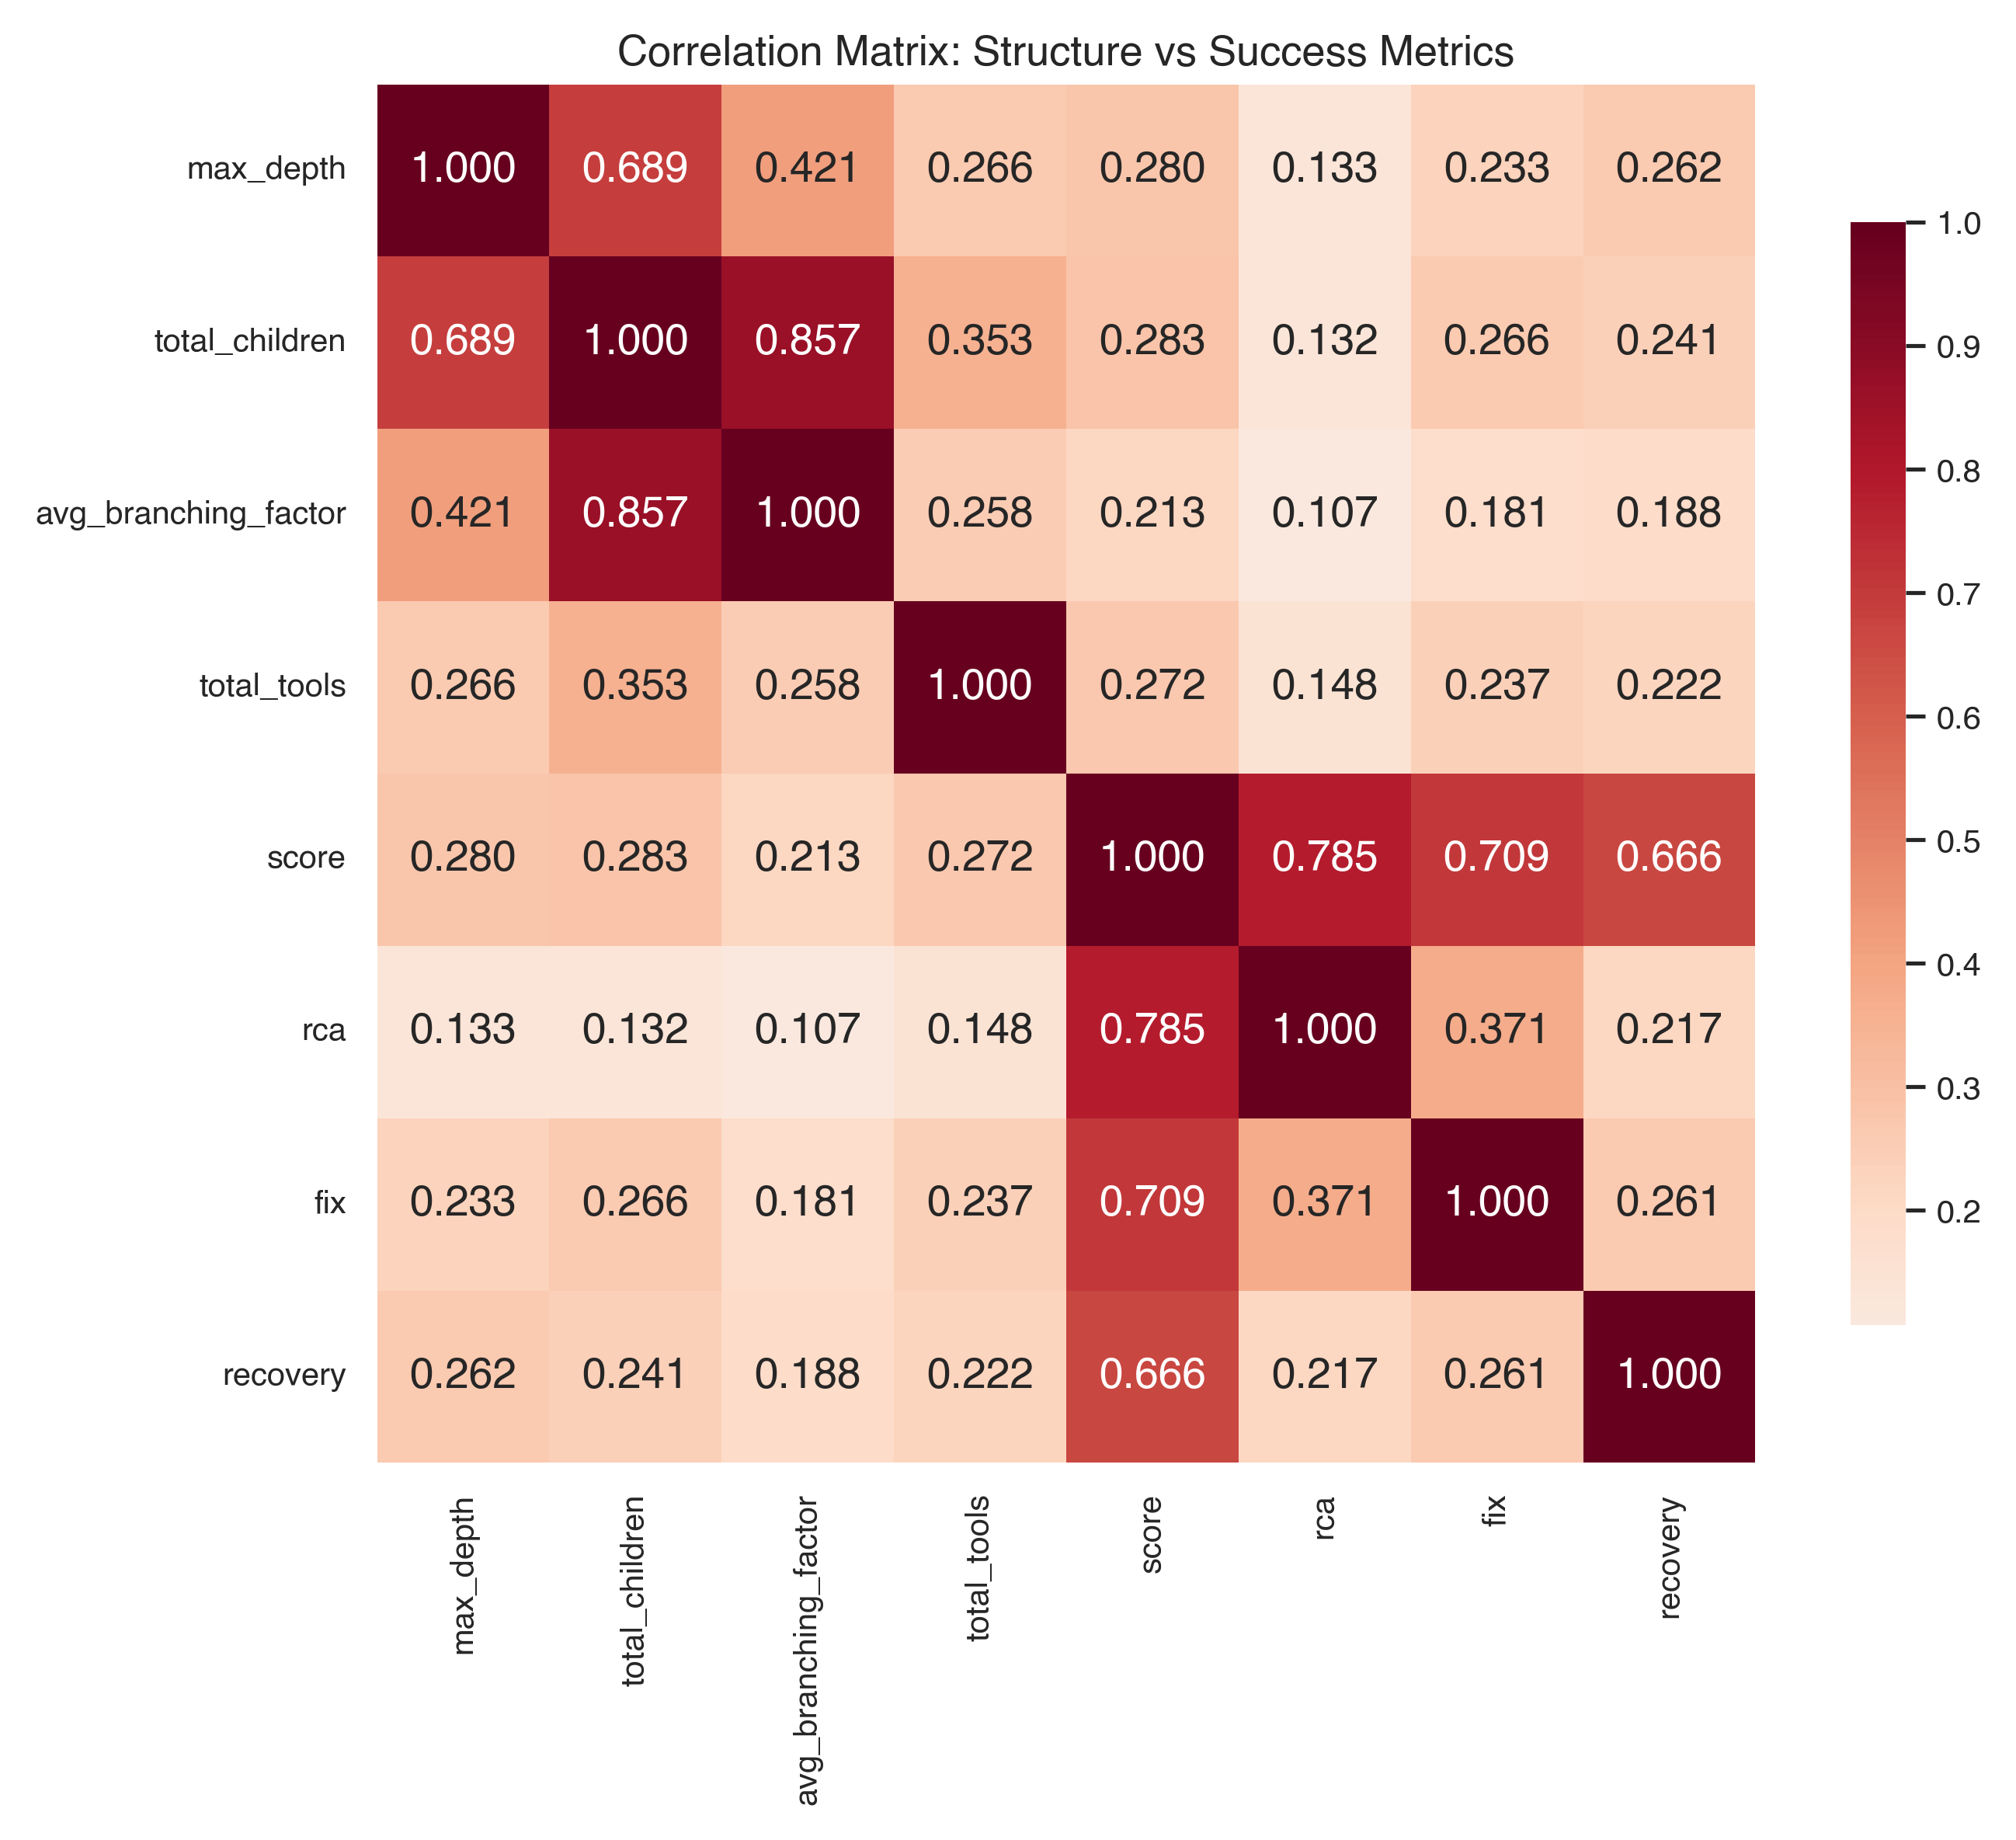
\includegraphics[width=0.8\textwidth]{grafika/wyniki/gpt_5_nano_100/figures/correlation_heatmap.png}
    \caption*{\footnotesize Źródło: opracowanie własne.}
\end{figure}

\begin{figure}[H]
    \centering
    \caption{Macierz korelacji dla modelu Minimax-2.5 (wariant z uczeniem). Widoczne są negatywne korelacje między total\_children (szerokość) a wskaźnikami sukcesu, odrzucając hipotezę H2 dla tego modelu.}
    \label{fig:correlation-heatmap-minimax}
    
\includegraphics[width=0.8\textwidth]{grafika/wyniki/minimax_25_100/figures/correlation_heatmap.png}
    \caption*{\footnotesize Źródło: opracowanie własne.}
\end{figure}

\paragraph{GPT-5-nano: Pełne potwierdzenie obu hipotez w wariancie z uczeniem.}
Model GPT-5-nano z aktywnym potokiem ACE wykazuje silne, statystycznie istotne korelacje pozytywne zarówno dla głębokości (r=0.316, p<0.001) jak i szerokości (r=0.351, p<0.001). Oznacza to, że agent wykorzystujący bogatszy Playbook systematycznie buduje głębsze i szersze drzewa zadań, a jednocześnie osiąga lepsze wyniki remediacji. W wariancie bez uczenia korelacje są słabsze i nieistotne statystycznie, co potwierdza, że strukturalne korzyści wynikają z ewolucji Playbooka, nie z bazowych właściwości modelu.

\paragraph{Minimax-2.5: Częściowe potwierdzenie z paradoksalną korelacją ujemną dla szerokości.}
Model Minimax-2.5 wykazuje istotnie odmienną charakterystykę. W wariancie z uczeniem hipoteza H1 (głębokość) została potwierdzona (r=0.143, p=0.045), ale hipoteza H2 (szerokość) została \textbf{odrzucona} z powodu ujemnej korelacji (r=-0.168, p=0.019). Oznacza to paradoks: większa szerokość drzewa zadań koreluje z \emph{gorszymi} wynikami. 

Ten wynik sugeruje, że Minimax-2.5 lepiej radzi sobie ze \emph{skoncentrowaną, sekwencyjną} analizą (mniej równoległych delegacji, ale głębsza hierarchia), podczas gdy GPT-5-nano skutecznie wykorzystuje \emph{rozproszoną, równoległą} organizację pracy (więcej jednoczesnych delegacji).

\paragraph{Implikacje dla projektowania systemów wieloagentowych.}
Te wyniki wskazują, że optymalna architektura systemu wieloagentowego jest silnie uzależniona od charakterystyk modelu językowego. Systemy oparte na modelach typu GPT mogą korzystać z szerokiej delegacji równoległej, podczas gdy modele typu Minimax wymagają bardziej linearnych, skoncentrowanych strategii działania.

\section{Analiza skuteczności w podziale na klasy incydentów}

Globalne uśrednienia maskują istotne zróżnicowanie wyników w obrębie poszczególnych klas usterek. Ze względu na różnice między modelami, analiza według klas incydentów zostanie przedstawiona osobno dla każdego modelu, z naciskiem na wzorce charakterystyczne dla Minimax-2.5, który wykazuje większe zróżnicowanie bazowe.

Szczegółowe wyniki w podziale na klasy incydentów dla obu modeli przedstawiono w tabelach~\ref{tab:by-incident-type-gpt5} i~\ref{tab:by-incident-type-minimax}. GPT-5-nano poprawia skuteczność we wszystkich czterech klasach, podczas gdy Minimax-2.5 wykazuje regresję wyłącznie w Klasie~1 (usterki hybrydowe).

\section{Chronologia procesu uczenia}

Aby zilustrować przebieg procesu uczenia, na rysunkach~\ref{fig:fig3-chronological-gpt5} i~\ref{fig:fig3-chronological-minimax} przedstawiono wskaźnik skuteczności remediacji każdego epizodu dla obu modeli, z zachowaniem chronologii ich uruchamiania. Takie zestawienie pozwala porównać wzorce uczenia reprezentowane przez oba modele. Każdy kolorowy słupek odpowiada pojedynczemu epizodowi, a kolor wskazuje uzyskaną punktację (zielony – 3 punkty, jasnozielony – 2 punkty, pomarańczowy – 1 punkt, czerwony – 0 punktów). Sekwencja epizodów jest identyczna w obu przypadkach. Dolny wykres przedstawia różnicę sumarycznej punktacji pomiędzy agentem korzystającym z potoku ACE (learning) a wariantem bez uczenia (Without learning).

\begin{figure}[H]
    \centering
    \caption{Chronologiczne porównanie wskaźników skuteczności remediacji poszczególnych epizodów dla modelu GPT-5-nano (skala 0--3). Górny pas: wariant bez uczenia (NL). Dolny pas: wariant z aktywnym potokiem ACE (L). Widoczny gwałtowny wzrost skuteczności w drugiej połowie eksperymentu po akumulacji wiedzy w Playbooku.}
    \label{fig:fig3-chronological-gpt5}
    
\includegraphics[width=\textwidth]{grafika/wyniki/gpt_5_nano_100/figures/fig3_chronological_timeline.png}
    \caption*{\footnotesize Źródło: opracowanie własne.}
\end{figure}

\begin{figure}[H]
    \centering
    \caption{Chronologiczne porównanie wskaźników skuteczności remediacji poszczególnych epizodów dla modelu Minimax-2.5 (skala 0--3). Górny pas: wariant bez uczenia (NL). Dolny pas: wariant z aktywnym potokiem ACE (L). Widoczna umiarkowana i równomierna poprawa w porównaniu do GPT-5-nano.}
    \label{fig:fig3-chronological-minimax}
    
\includegraphics[width=\textwidth]{grafika/wyniki/minimax_25_100/figures/fig3_chronological_timeline.png}
    \caption*{\footnotesize Źródło: opracowanie własne.}
\end{figure}

W przypadku wariantu bez uczenia, dla obu modeli rozkład punktacji pozostaje stacjonarny - nie zaobserwowano systematycznego wzrostu skuteczności w miarę postępu eksperymentu. Potwierdza to, że pojedyncze instancje agenta SRE nie dzielą się doświadczeniem pomiędzy epizodami.

W wariancie z aktywnym potokiem ACE widać wyraźne różnice pomiędzy modelami:
\begin{itemize}
    \item \textbf{GPT-5-nano}: Zauważalny jest wyraźny postęp - w drugiej połowie eksperymentu występuje dramatyczny wzrost skuteczności oraz koncentracja epizodów z wysoką punktacją ($\geq$2).
    \item \textbf{Minimax-2.5}: Postęp poprawy jest bardziej równomierny i umiarkowany na przestrzeni całego eksperymentu.
\end{itemize}

Taki efekt można powiązać z momentami synchronizacji Playbooka, które odbywały się co 5 epizodów. GPT-5-nano wykazuje szczególnie wysoką zdolność do wykorzystania akumulującej się wiedzy proceduralnej.

\section{Ewolucja Playbooka: rozmiar, liczba reguł i dystrybucja wiedzy pomiędzy agentami}
\label{sec:ewolucja-playbooka}

Aby zobrazować dynamikę narastania bazy wiedzy proceduralnej w wariancie z aktywnym potokiem ACE, na rysunkach~\ref{fig:fig5-playbook-evolution-gpt5} i~\ref{fig:fig5-playbook-evolution-minimax} przedstawiono ewolucję Playbooka dla obu modeli pomiędzy kolejnymi rewizjami. Każda rewizja odpowiada jednemu uruchomieniu cyklu \textit{Reflektor}--\textit{Kurator}, wykonywanemu zgodnie ze strategią \textit{batch learning} co 5 epizodów.

\begin{figure}[H]
    \centering
    \caption{Ewolucja Playbooka dla modelu GPT-5-nano w trakcie eksperymentu z aktywnym potokiem ACE. Górny panel: łączny rozmiar Playbooka w tokenach z dekompozycją na cztery role agentowe. Dolny panel: liczba reguł IF/THEN per agent w kolejnych rewizjach.}
    \label{fig:fig5-playbook-evolution-gpt5}
    
\includegraphics[width=\textwidth]{grafika/wyniki/gpt_5_nano_100/figures/fig5_playbook_evolution.png}
    \caption*{\footnotesize Źródło: opracowanie własne.}
\end{figure}

\begin{figure}[H]
    \centering
    \caption{Ewolucja Playbooka dla modelu Minimax-2.5 w trakcie eksperymentu z aktywnym potokiem ACE. Górny panel: łączny rozmiar Playbooka w tokenach z dekompozycją na cztery role agentowe. Dolny panel: liczba reguł IF/THEN per agent w kolejnych rewizjach.}
    \label{fig:fig5-playbook-evolution-minimax}
    
\includegraphics[width=\textwidth]{grafika/wyniki/minimax_25_100/figures/fig5_playbook_evolution.png}
    \caption*{\footnotesize Źródło: opracowanie własne.}
\end{figure}

Z analizy wykresu wynika kilka istotnych obserwacji jakościowych.

Po pierwsze, \textbf{łączny rozmiar Playbooka rośnie blisko trzykrotnie} - z 1\,546 tokenów w rewizji początkowej do 4\,355 tokenów w rewizji końcowej (+182\%). Wzrost ma charakter zasadniczo monotoniczny, z niewielkim chwilowym spadkiem pomiędzy \textit{Rev~0} a \textit{Rev~1} (1\,546 $\to$ 1\,380~tokenów), który należy interpretować jako efekt pierwszej konsolidacji przez \textit{Kuratora}, eliminującej duplikaty i nadmiarowe sformułowania w bazowych regułach inicjalnych. Pojedynczy lokalny plateau w okolicy \textit{Rev~6}--\textit{Rev~7} (3\,732~$\to$~3\,739~tokenów) sugeruje moment, w którym kolejne refleksje były głównie absorbowane przez modyfikację istniejących reguł, a nie poprzez ich namnażanie.

Po drugie, \textbf{dystrybucja wiedzy pomiędzy agentami nie jest jednorodna}. \textit{Monitoring Agent} dysponuje konsekwentnie największą liczbą reguł - jego Playbook startuje z 21~reguł i osiąga 35~reguł w \textit{Rev~9}. Świadczy to o szczególnej gęstości wiedzy proceduralnej dotyczącej obserwowalności (interpretacja metryk Prometheusa, kwerendy LogQL, korelacja sygnałów z różnych źródeł).

Po trzecie, agenci \textit{Incident Commander}, \textit{DevOps Agent} oraz \textit{Coder Agent} startują z porównywalnie skromnym Playbookiem (8--20~reguł) i wszystkie trzy bazy wiedzy w toku eksperymentu wzrastają do poziomu 20--27~reguł. Najbardziej dynamiczny przyrost obserwujemy dla \textit{DevOps Agenta} (8~$\to$~27, +237\%), co dobrze koreluje z dwoma niezależnymi wynikami przedstawionymi wcześniej: skokiem skuteczności w Klasie~3 (błędna konfiguracja Kubernetes, $+200\%$) oraz wzrostem liczby błędów wywołań \texttt{kubectl\_exec} ($+185,3\%$). Obie te zmiany są napędzane przez nowe heurystyki dotyczące weryfikacji konfiguracji wewnątrz kontenerów, które rezydują właśnie w Playbooku \textit{DevOps Agenta}.

Po czwarte, \textbf{tempo przyrostu reguł nie pokrywa się dokładnie z tempem przyrostu tokenów}. W szczególności pomiędzy \textit{Rev~6} a \textit{Rev~7} liczba reguł \textit{Monitoring Agenta} spada z 34~do~31, podczas gdy łączny rozmiar Playbooka pozostaje praktycznie niezmieniony. Wskazuje to na operację \emph{kompresji semantycznej} wykonywaną przez \textit{Kuratora}: kilka pokrewnych reguł zostało scalonych w mniej liczne, lecz dłuższe i bardziej ogólne sformułowania - dokładnie taka operacja ujawnia się w surowych snapshotach (zob. wizualizacja kolorystyczna w \texttt{viz\_playbook\_evolution.py}, gdzie reguły powstałe w późnych fazach przejmują semantykę kilku reguł wcześniejszych).

Z perspektywy pytania badawczego nr~2 dotyczącego kosztu operacyjnego, należy odnotować praktyczną konsekwencję obserwowanego wzrostu: trzykrotnie większy Playbook oznacza trzykrotnie większy stały narzut tokenowy w każdej iteracji każdego agenta. Przy oknie kontekstowym 204\,800~tokenów wykorzystywanego modelu MiniMax-M2 (zob. tabela~\ref{tab:agent-config}) finalny rozmiar 4\,355~tokenów stanowi nieco ponad 2\% dostępnej puli, co pozostawia bezpieczny margines, ale jednocześnie wskazuje na potencjalny problem skalowalności w dłuższych eksperymentach - temat ten jest podejmowany w Rozdziale~VII jako kierunek dalszych prac dotyczący warunkowanej selekcji reguł Playbooka.

\section{Metryki operacyjne}

Analiza efektywności operacyjnej - czasu naprawy, liczby iteracji, intensywności wywołań narzędzi oraz głębokości struktury drzewa zadań została przeprowadzona dla obu modeli. Wyniki przedstawiono na rysunkach~\ref{fig:fig2-operational-gpt5} i~\ref{fig:fig2-operational-minimax}, ilustrujących różne profile kompromisu skuteczność vs złożoność.

\begin{figure}[H]
    \centering
    \caption{Rozkłady metryk operacyjnych dla modelu GPT-5-nano (wykresy pudełkowe nałożone na wykresy skrzypcowe). Górny rząd: czas do rozwiązania (TTR), długość trajektorii konwersacji, liczba iteracji w korzeniu drzewa. Dolny rząd: liczba wywołań narzędzi, odsetek błędów wywołań, maksymalna głębokość drzewa zadań.}
    \label{fig:fig2-operational-gpt5}
    
\includegraphics[width=\textwidth]{grafika/wyniki/gpt_5_nano_100/figures/fig2_operational_comparison.png}
    \caption*{\footnotesize Źródło: opracowanie własne.}
\end{figure}

\begin{figure}[H]
    \centering
    \caption{Rozkłady metryk operacyjnych dla modelu Minimax-2.5 (wykresy pudełkowe nałożone na wykresy skrzypcowe). Górny rząd: czas do rozwiązania (TTR), długość trajektorii konwersacji, liczba iteracji w korzeniu drzewa. Dolny rząd: liczba wywołań narzędzi, odsetek błędów wywołań, maksymalna głębokość drzewa zadań. Widoczny wzrost złożoności w wariancie z uczeniem przy umiarkowanej poprawie skuteczności.}
    \label{fig:fig2-operational-minimax}
    
\includegraphics[width=\textwidth]{grafika/wyniki/minimax_25_100/figures/fig2_operational_comparison.png}
    \caption*{\footnotesize Źródło: opracowanie własne.}
\end{figure}

\begin{table}[H]
    \centering
    \caption{Metryki operacyjne (mediana / średnia) dla obu wariantów. Wartość $\Delta$ średniej obliczona jako różnica L $-$ NL.}
    \label{tab:operational-metrics}
    \footnotesize
    \begin{tabular}{lccr}
        \hline
        \textbf{Metryka}                     & \textbf{Bez uczenia}     & \textbf{Z uczeniem}      & \textbf{$\Delta$ średniej} \\
        \hline
        TTR (min, korzeń)                    & 10,6 / 12,3              & 11,9 / 11,9              & $-$0,4 min ($-$2,9\%) \\
        Długość trajektorii (wszystkie)      & 41,0 / 43,1              & 41,0 / 43,3              & +0,2 (+0,4\%) \\
        Liczba iteracji (korzeń)             & 12,0 / 15,4              & 25,0 / 26,1              & +10,7 (+69,9\%) \\
        Liczba wywołań narzędzi (wszystkie)  & 20,0 / 21,0              & 20,0 / 20,9              & $-$0,1 ($-$0,5\%) \\
        Odsetek błędnych wywołań             & 6,2\% / 8,6\%            & 8,0\% / 10,2\%           & +1,6 pp (+18,9\%) \\
        Maks. głębokość drzewa (korzeń)      & 1,00 / 1,02              & 1,00 / 1,29              & +0,27 (+26,1\%) \\
        Łączna liczba potomków (korzeń)      & 4,0 / 4,1                & 4,0 / 4,5                & +0,4 (+10,3\%) \\
        \hline
    \end{tabular}
    \caption*{\footnotesize Źródło: opracowanie własne.}
\end{table}

Interpretacja wyników operacyjnych prowadzi do nietrywialnego wniosku: \textbf{poprawa skuteczności okupiona została wzrostem złożoności obliczeniowej}, a nie jej redukcją. Średnia liczba iteracji w korzeniu drzewa rośnie o $+69,9\%$ (z 15,4 do 26,1), maksymalna głębokość drzewa o $+26,1\%$, a odsetek błędnych wywołań narzędzi rośnie o $+1,6$ punktu procentowego.

Zjawisko to można wyjaśnić w kategoriach \textit{eksploracji vs eksploatacji}: agenci wyposażeni w bogatszy Playbook podejmują więcej kroków diagnostycznych przed sformułowaniem hipotezy, częściej delegują podzadania do wyspecjalizowanych agentów (\textit{Monitoring Agent}, \textit{DevOps Agent}, \textit{Coder Agent}) i częściej wykonują weryfikację stanu klastra po wprowadzeniu zmiany. Każda z tych dodatkowych operacji zwiększa liczbę iteracji oraz szansę na pojedynczy błąd narzędziowy, ale jednocześnie istotnie zwiększa końcowe prawdopodobieństwo skutecznej remediacji.

Co istotne, mimo wzrostu liczby iteracji o blisko 70\%, \textbf{średni czas TTR uległ niewielkiemu spadkowi} ($-$2,9\%, z 12,3~min do 11,9~min). Oznacza to, że dodatkowe iteracje są realizowane znacznie szybciej - dzięki bardziej precyzyjnym instrukcjom z Playbooka agenci nie marnują czasu na ślepe próby wywołań narzędzi z błędnymi parametrami, lecz wykonują skoncentrowane, krótkie kroki weryfikacyjne. Mediana TTR w wariancie z uczeniem (11,9~min) jest natomiast nieznacznie wyższa od mediany NL (10,6~min), co wskazuje na zwiększenie spójności rozkładu czasu naprawy (mniej epizodów ekstremalnie krótkich i ekstremalnie długich).

\section{Emergentna organizacja pracy: pogłębienie drzewa zadań i intensyfikacja delegacji}
\label{sec:emergentna-organizacja}

Najciekawszą emergentną właściwością obserwowaną w wariancie z aktywnym potokiem ACE jest jakościowa zmiana struktury \textit{drzewa zadań} (\textit{tasks tree}) generowanego przez \textit{Incident Commandera}. Ze względu na różne charakterystyki strukturalne między modelami, przedstawiono wyniki dla obu modeli (rysunki~\ref{fig:fig6-tree-structure-gpt5} i~\ref{fig:fig6-tree-structure-minimax}), które ilustrują odmienne wzorce organizacji pracy.

\begin{figure}[H]
    \centering
    \caption{Statystyki struktury drzewa zadań dla modelu GPT-5-nano. Lewy górny: średnia liczba dzieci per poziom (Depth~1, Depth~2). Prawy górny: średnia łączna liczba potomków oraz maksymalna głębokość. Dolny rząd: rozkłady liczby dzieci na poziomach 1 i 2 (wykresy skrzypcowe). Widoczne zwiększenie zarówno głębokości jak i szerokości w wariancie z uczeniem.}
    \label{fig:fig6-tree-structure-gpt5}
    
\includegraphics[width=\textwidth]{grafika/wyniki/gpt_5_nano_100/figures/fig6_tree_structure.png}
    \caption*{\footnotesize Źródło: opracowanie własne.}
\end{figure}

\begin{figure}[H]
    \centering
    \caption{Statystyki struktury drzewa zadań dla modelu Minimax-2.5. Lewy górny: średnia liczba dzieci per poziom (Depth~1, Depth~2). Prawy górny: średnia łączna liczba potomków oraz maksymalna głębokość. Dolny rząd: rozkłady liczby dzieci na poziomach 1 i 2 (wykresy skrzypcowe). Widoczne mniejsze zmiany w strukturze w porównaniu do GPT-5-nano.}
    \label{fig:fig6-tree-structure-minimax}
    
\includegraphics[width=\textwidth]{grafika/wyniki/minimax_25_100/figures/fig6_tree_structure.png}
    \caption*{\footnotesize Źródło: opracowanie własne.}
\end{figure}

\begin{figure}[H]
    \centering
    \caption{Przykład rozbudowanego drzewa epizodu wygenerowanego w wariancie z aktywnym potokiem ACE, ilustrujący pogłębienie struktury delegacji na poziomie~2: agent pośredni rekursywnie deleguje podzadania do pozostałych agentów, realizując wieloetapową analizę w paradygmacie agent-jako-narzędzie.}
    \label{fig:przyklad-rozbudowanego-drzewa}
    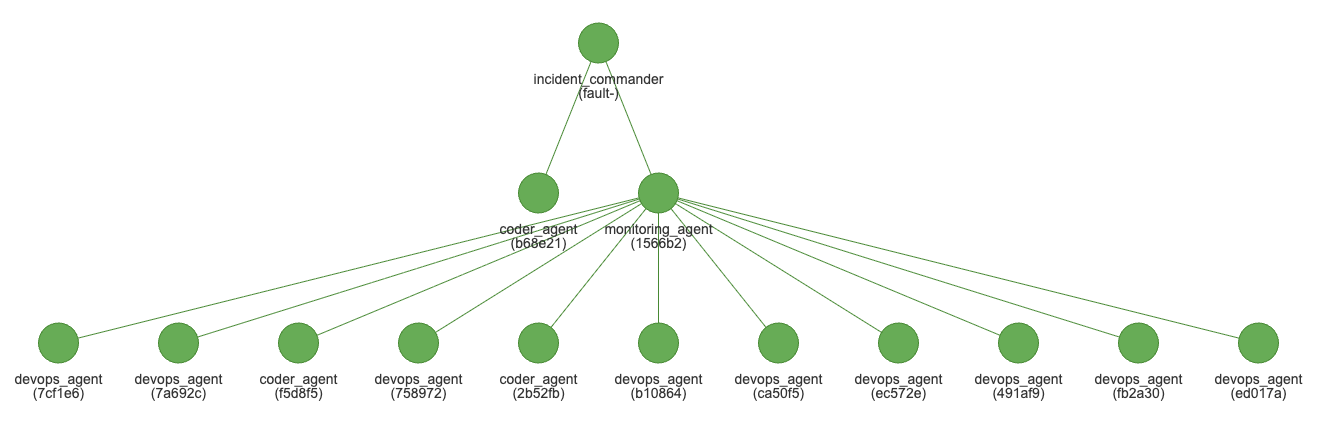
\includegraphics[width=\textwidth]{grafika/przyklad-rozbudowanego-drzewa.png}
    \caption*{\footnotesize Źródło: opracowanie własne. Epizod \texttt{fault-4-mongo-553578c6-e7ed-40ce-a43c-b00e7a4750a2}, model Minimax-2.5 z uczeniem (baza \texttt{minimax\_25\_100/agent.db}).}
\end{figure}

Najbardziej znamienna jest zmiana na poziomie \textbf{drugim} drzewa - średnia liczba dzieci na tym poziomie wzrasta z 0,2 (NL) do 0,8 (L), a odsetek epizodów posiadających jakiekolwiek zadania na poziomie 2 wzrasta z 13\% do 30\%. Oznacza to, że w wariancie z uczeniem rośnie liczba sytuacji, w których agent średniego szczebla sam staje się delegatorem, dzieląc swoje zadanie na dalsze podzadania - co ilustruje rysunek~\ref{fig:przyklad-rozbudowanego-drzewa}.

Zjawisko to bezpośrednio potwierdza trzecią hipotezę postawioną w Rozdziale~V dotyczącą \emph{emergentnej organizacji pracy}: system wieloagentowy uczy się wzorców wieloetapowej, hierarchicznej delegacji bez konieczności jawnego programowania takiej strategii. Heurystyki zapisane w Playbookach poszczególnych ról (zwłaszcza w Playbooku \textit{Incident Commandera}) zaczynają częściej zalecać schemat: \emph{najpierw zleć analizę metryk, dopiero potem na jej podstawie deleguj fix do DevOps lub Coder Agenta}, co skutkuje pojawieniem się głębszych poddrzew. Średnia maksymalna głębokość drzewa wzrasta z 1,02 do 1,29, co przy ograniczeniu architektonicznym wynoszącym maksymalnie 3 poziomy (opisanym w Rozdziale~III) oznacza istotne wykorzystanie tej swobody projektowej.

Należy jednak podkreślić, że na poziomie \textbf{pierwszym} (bezpośrednie dzieci \textit{Incident Commandera}) średnia liczba delegacji praktycznie się nie zmienia (3,9 vs 3,8). Świadczy to o tym, że ewolucja Playbooka nie zwiększa rozproszenia pracy na najwyższym szczeblu organizacyjnym (gdzie zachowana jest stabilna, czteroelementowa pula deputatów), lecz jakościowo modyfikuje sposób pracy poszczególnych agentów, którzy po otrzymaniu zadania częściej decydują o uruchomieniu własnego procesu rekursywnej delegacji.

\section{Analiza błędów wywołań narzędzi}

Ostatni, zaobserwowany wymiar zmiany dotyczy struktury błędów wywołań narzędzi. Choć globalny odsetek błędów wzrasta (zob. tabela~\ref{tab:operational-metrics}), to jego wewnętrzny profil ulega istotnemu przetasowaniu - wyniki przedstawiono na rysunku~\ref{fig:fig4-failing-tools-minimax} oraz w tabeli~\ref{tab:failing-tools}.

\begin{figure}[H]
    \centering
    \caption{Bezwzględna liczba błędnych wywołań w podziale na narzędzia dla modelu Minimax-2.5 (wykresy poziome posortowane według liczby błędów w wariancie L). Wybrano ten model ze względu na wyraźne wzorce zmian w profilach błędów między wariantami.}
    \label{fig:fig4-failing-tools-minimax}
    
\includegraphics[width=\textwidth]{grafika/wyniki/minimax_25_100/figures/fig4_failing_tools.png}
    \caption*{\footnotesize Źródło: opracowanie własne.}
\end{figure}

\begin{table}[H]
    \centering
    \caption{Top-10 narzędzi o największej liczbie błędnych wywołań. Wartość $\Delta$ jest różnicą bezwzględną i względną pomiędzy wariantami.}
    \label{tab:failing-tools}
    \footnotesize
    \begin{tabular}{lrrr}
        \hline
        \textbf{Narzędzie}                                  & \textbf{NL}  & \textbf{L}   & \textbf{$\Delta$ (L $-$ NL)} \\
        \hline
        \texttt{execute\_code}                              & 205          & 212          & +7 (+3,4\%) \\
        \texttt{kubectl\_exec}                              & 68           & 194          & +126 (+185,3\%) \\
        \texttt{bash}                                       & 89           & 54           & $-$35 ($-$39,3\%) \\
        \texttt{kubectl\_get\_resources}                    & 59           & 48           & $-$11 ($-$18,6\%) \\
        \texttt{kubectl\_get\_resource}                     & 14           & 13           & $-$1 ($-$7,1\%) \\
        \texttt{kubectl\_get\_yaml}                         & 13           & 4            & $-$9 ($-$69,2\%) \\
        \texttt{kubectl\_rollout\_status}                   & 7            & 7            & 0 (0,0\%) \\
        \texttt{get\_list\_code\_definitions\_names\_descriptions} & 1     & 12           & +11 (+1100,0\%) \\
        \texttt{read\_file}                                 & 5            & 6            & +1 (+20,0\%) \\
        \texttt{kubectl\_describe}                          & 7            & 3            & $-$4 ($-$57,1\%) \\
        \hline
        \textbf{Łącznie (wszystkie narzędzia)}              & \textbf{513} & \textbf{611} & \textbf{+98 (+19,1\%)} \\
        \hline
    \end{tabular}
    \caption*{\footnotesize Źródło: opracowanie własne.}
\end{table}

Profil błędów ujawnia dwa przeciwstawne zjawiska. Po pierwsze, w wariancie z uczeniem widoczny jest \textbf{istotny spadek błędów dla narzędzi ogólnego przeznaczenia}: \texttt{bash} ($-$39,3\%), \texttt{kubectl\_get\_yaml} ($-$69,2\%), \texttt{kubectl\_describe} ($-$57,1\%), \texttt{kubectl\_get\_resources} ($-$18,6\%). Reguły IF/THEN w Playbookach zawierają precyzyjne wzorce wywołań tych narzędzi (właściwe \texttt{namespace}, format selektorów, oczekiwany typ zasobu), co eliminuje halucynacje parametrów typowe dla agenta nieuzbrojonego w wiedzę proceduralną.

Po drugie, obserwujemy \textbf{wyraźny wzrost błędów dla \texttt{kubectl\_exec} ($+185,3\%$)}. Wynika to z faktu, że nowe heurystyki w Playbooku \textit{DevOps Agenta} aktywnie zachęcają do wykonywania interaktywnych sesji wewnątrz kontenerów (np. w celu walidacji konfiguracji aplikacji w runtime). Narzędzie \texttt{kubectl\_exec} jest jednak wewnętrznie zawodne - wymaga, aby docelowy pod był w stanie \texttt{Running}, a kontener pozostawał responsywny. W incydentach Klasy~1 i Klasy~3 (gdzie pod znajduje się często w stanie \texttt{Pending} lub \texttt{CrashLoopBackOff}) ta strategia generuje liczne, lecz proceduralnie poprawne błędy zwrotne. Mechanizm ten wyjaśnia również częściową regresję w Klasie~1 zauważoną w tabeli~\ref{tab:by-incident-type-minimax}.

Łączna liczba błędów wywołań rośnie z 513 do 611 ($+19,1\%$), ale liczba ta musi być zestawiana z prawie 70\% wzrostem liczby iteracji. Po normalizacji \emph{względny} odsetek błędów rośnie tylko o 1,6 punktu procentowego (z 8,6\% do 10,2\%), co przy jednoczesnym wzroście wskaźnika \texttt{system\_recovery\_visible} o $+60\%$ uznać należy za korzystny kompromis.

\section{Analiza wzorców emergentnych: sekwencje n-gramowe delegacji i narzędzi}

Jedną z najbardziej wartościowych metod analizy emergentnej organizacji pracy w systemie wieloagentowym jest badanie wzorców n-gramowych - sekwencji kolejnych delegacji zadań oraz wywołań narzędzi. Analiza ta pozwala zidentyfikować powtarzalne strategie działania, które spontanicznie wykształciły się w wariancie z aktywnym potokiem ACE.

\subsection{Metodyka analizy n-gramowej}

Analiza n-gramowa opisana w podsekcjach~\ref{subsec:wzorce-gpt} i~\ref{subsec:wzorce-minimax} została przeprowadzona wyłącznie na wariancie z uczeniem (\textbf{L}). Wzorce zidentyfikowane w tych podsekcjach opisują zatem charakterystykę agenta \emph{po} aktywacji potoku ACE. Pytanie, czy wzorce te są \emph{emergentne} - tzn. czy pojawiły się wskutek uczenia - jest odpowiadane osobno w podsekcji~\ref{subsec:emergencja-dynamika}, gdzie każdy wzorzec jest porównywany z jego odpowiednikiem w wariancie NL (analiza $\Delta$lift) oraz śledzona jego ewolucja w czasie (podział L1/L2).

Analiza n-gramowa przeprowadzona w niniejszej pracy wprowadza dwa kluczowe założenia metodologiczne.

\textbf{Jednostka analizy: epizod, nie wystąpienie.} Ten sam n-gram może pojawić się wielokrotnie w ramach jednego epizodu - np. pięć kolejnych delegacji do \texttt{coder\_agent} generuje cztery wystąpienia 2-gramu \texttt{coder→coder}. Zliczanie wystąpień zamiast epizodów zawyżałoby skuteczność wzorców obecnych w epizodach zakończonych wieloma nieudanymi próbami. W przyjętym podejściu każdy epizod jest klasyfikowany binarnie: wzorzec jest w nim obecny lub nie. Wskaźnik sukcesu wzorca to odsetek epizodów z danym wzorcem, które zakończyły się sukcesem (score~$\geq$~2).

\textbf{Lift ponad bazową skuteczność.} Surowy wskaźnik sukcesu wzorca jest miarą nieporównywalną między modelami o różnej skuteczności bazowej. Stosowaną miarą jest lift:
\[
  \mathrm{lift}(W) = \frac{P(\text{sukces} \mid \text{wzorzec } W \text{ obecny})}{P(\text{sukces})}
\]
Lift $> 1{,}0$ oznacza, że wzorzec koreluje z sukcesem; lift $< 1{,}0$ - z porażką. Dla każdego wzorca przeprowadzono dwustronny test dokładny Fishera na tabeli $2 \times 2$ (epizody z/bez wzorca $\times$ sukces/porażka). Raportowane są wzorce z minimalną licznością $n \geq 5$ epizodów. Skuteczności bazowe: GPT-5-nano 33,7\% (33/98 epizodów), Minimax-2.5 43,9\% (43/98 epizodów).

\subsection{Wzorce GPT-5-nano}
\label{subsec:wzorce-gpt}

\begin{table}[H]
    \centering
    \caption{Wzorce n-gramowe istotne statystycznie dla modelu GPT-5-nano (wariant z uczeniem, $p < 0{,}05$). Wzorce pogrupowane według kategorii i posortowane malejąco według lift.}
    \label{tab:ngrams-gpt5}
    \footnotesize
    \begin{tabular}{p{0.50\textwidth}cccc}
        \hline
        \textbf{Wzorzec} & \textbf{Lift} & \textbf{Sukces} & \textbf{n} & \textbf{p} \\
        \hline
        \multicolumn{5}{l}{\textit{2-gramy delegacji korelujące z sukcesem:}} \\[2pt]
        \texttt{monitoring\_agent $\to$ coder\_agent}            & 1,55 & 52,3\%  & 44 & $<0{,}001^{***}$ \\
        \texttt{devops\_agent $\to$ monitoring\_agent}           & 1,46 & 49,0\%  & 51 & $0{,}001^{**}$ \\
        \texttt{coder\_agent $\to$ devops\_agent}                & 1,31 & 44,2\%  & 52 & $0{,}031^{*}$ \\
        \texttt{monitoring\_agent $\to$ devops\_agent}           & 1,29 & 43,4\%  & 53 & $0{,}033^{*}$ \\
        \hline
        \multicolumn{5}{l}{\textit{3-gramy delegacji korelujące z sukcesem:}} \\[2pt]
        \texttt{monitoring $\to$ coder $\to$ coder}              & 2,97 & 100,0\% & 5  & $0{,}004^{**}$ \\
        \texttt{devops $\to$ monitoring $\to$ devops}            & 2,16 & 72,7\%  & 11 & $0{,}006^{**}$ \\
        \texttt{monitoring $\to$ coder $\to$ devops}             & 1,78 & 60,0\%  & 25 & $0{,}003^{**}$ \\
        \texttt{devops $\to$ monitoring $\to$ coder}             & 1,52 & 51,3\%  & 39 & $0{,}004^{**}$ \\
        \hline
        \multicolumn{5}{l}{\textit{Wzorce narzędziowe korelujące z sukcesem:}} \\[2pt]
        \texttt{read\_file $\to$ read\_file $\to$ assign\_task}  & 1,75 & 58,8\%  & 17 & $0{,}023^{*}$ \\
        \texttt{assign\_task $\to$ assign\_task}                 & 1,25 & 42,1\%  & 76 & $<0{,}001^{***}$ \\
        \hline
        \multicolumn{5}{l}{\textit{Wzorzec korelujący z porażką:}} \\[2pt]
        \texttt{monitoring\_agent $\to$ monitoring\_agent}       & 0,00 & 0,0\%   & 8  & $0{,}049^{*}$ \\
        \hline
    \end{tabular}
    \caption*{\footnotesize Źródło: opracowanie własne.}
\end{table}

\subsection{Wzorce Minimax-2.5}
\label{subsec:wzorce-minimax}

\begin{table}[H]
    \centering
    \caption{Wzorce n-gramowe istotne statystycznie dla modelu Minimax-2.5 (wariant z uczeniem, $p < 0{,}05$). Wzorce pogrupowane według kategorii i posortowane malejąco według lift.}
    \label{tab:ngrams-minimax}
    \footnotesize
    \begin{tabular}{p{0.50\textwidth}cccc}
        \hline
        \textbf{Wzorzec} & \textbf{Lift} & \textbf{Sukces} & \textbf{n} & \textbf{p} \\
        \hline
        \multicolumn{5}{l}{\textit{Wzorzec delegacji korelujący z sukcesem:}} \\[2pt]
        \texttt{coder\_agent $\to$ monitoring\_agent}                    & 1,50 & 65,9\% & 41 & $<0{,}001^{***}$ \\
        \hline
        \multicolumn{5}{l}{\textit{Wzorce narzędziowe korelujące z sukcesem:}} \\[2pt]
        \texttt{read\_file $\to$ update\_todo $\to$ deploy\_app}         & 1,95 & 85,7\% & 14 & $<0{,}001^{***}$ \\
        \texttt{update\_todo $\to$ deploy\_app}                          & 1,68 & 73,9\% & 23 & $0{,}002^{**}$ \\
        \texttt{update\_todo $\to$ deploy\_app $\to$ assign\_task}       & 1,63 & 71,4\% & 21 & $0{,}006^{**}$ \\
        \texttt{deploy\_app $\to$ assign\_task}                          & 1,60 & 70,3\% & 37 & $<0{,}001^{***}$ \\
        \texttt{deploy\_app $\to$ assign\_task $\to$ update\_todo}       & 1,52 & 66,7\% & 24 & $0{,}017^{*}$ \\
        \hline
        \multicolumn{5}{l}{\textit{Wzorce delegacji korelujące z porażką:}} \\[2pt]
        \texttt{devops $\to$ monitoring $\to$ monitoring}                & 0,14 & 6,2\%  & 16 & $<0{,}001^{***}$ \\
        \texttt{monitoring $\to$ monitoring $\to$ devops}                & 0,15 & 6,7\%  & 15 & $0{,}001^{**}$ \\
        \texttt{devops $\to$ devops $\to$ devops}                        & 0,30 & 13,3\% & 15 & $0{,}011^{*}$ \\
        \texttt{monitoring $\to$ devops $\to$ devops}                    & 0,42 & 18,5\% & 27 & $0{,}003^{**}$ \\
        \texttt{monitoring\_agent $\to$ monitoring\_agent}               & 0,49 & 21,4\% & 28 & $0{,}006^{**}$ \\
        \texttt{devops\_agent $\to$ devops\_agent}                       & 0,49 & 21,4\% & 28 & $0{,}006^{**}$ \\
        \hline
    \end{tabular}
    \caption*{\footnotesize Źródło: opracowanie własne.}
\end{table}

\subsection{Interpretacja różnic w strategiach}
\label{subsec:interpretacja}

Analiza oparta na lifcie ujawnia jakościowo odmienną strukturę wzorców niż podejście oparte wyłącznie na surowym wskaźniku sukcesu.

\textbf{GPT-5-nano: delegacja cyrkulacyjna.} Wszystkie cztery istotne statystycznie wzorce 2-gramowe delegacji to przejścia \emph{między różnymi agentami}: \texttt{monitoring→coder}, \texttt{devops→monitoring}, \texttt{coder→devops}, \texttt{monitoring→devops}. Jedynym 2-gramem korelującym z porażką jest \texttt{monitoring→monitoring} (lift~0,00, $p < 0{,}05$) - ponowne zlecenie zadania temu samemu agentowi jest sygnałem niepowodzenia. Wzorce 3-gramowe potwierdzają ten schemat: najskuteczniejsze sekwencje to cyrkulacje między agentami (\texttt{devops→monitoring→devops}, lift~2,16; \texttt{monitoring→coder→devops}, lift~1,78). Wzorzec na poziomie narzędzi \texttt{assign\_task→assign\_task} (lift~1,25, $p < 0{,}001$) potwierdza, że sama seria kolejnych delegacji jest dla GPT-5-nano operacyjnie korzystna.

\textbf{Minimax-2.5: weryfikacja i zamknięcie cyklu remediacji.} Jedynym istotnym wzorcem delegacyjnym jest \texttt{coder→monitoring} (lift~1,50, $p < 0{,}001$). Natomiast sekwencje delegacji między Monitoring Agent a DevOps Agent są silnymi predyktorami porażki: sześć wzorców (2- i 3-gramowych) osiąga istotność statystyczną poniżej bazy, z czego dwa mają lift $< 0{,}2$ przy $p < 0{,}001$. Wzorce sukcesu leżą w sekwencjach narzędziowych prowadzących do wdrożenia: \texttt{update\_todo $\to$ deploy\_app} (lift~1,68) i \texttt{read\_file $\to$ update\_todo $\to$ deploy\_app} (lift~1,95). Należy jednak podkreślić, że sekwencja \texttt{read\_file $\to$ update\_todo $\to$ deploy\_app} stanowi \emph{mechaniczny artefakt aktu wdrożenia}, nie wyróżniającą się strategię organizacyjną: każdy agent implementujący naprawę musi zweryfikować stan pliku, zaktualizować status zadania i wywołać deployment. Wysoki lift tej sekwencji jest częściowo tautologiczny - sukces wymaga wdrożenia, więc sekwencje narzędziowe prowadzące do wdrożenia korelują z sukcesem z definicji. Faktycznym odkryciem jest co innego: ACE uczy Minimax-2.5 \emph{unikania pętli diagnostycznych} (monitoring$\leftrightarrow$devops, lift~$<0{,}2$) i \emph{zamykania cyklu remediacji} przez wdrożenie, zamiast przerywania go w fazie diagnozy.

\paragraph{Asymetria jakościowa: koordynacja agentów vs zamknięcie cyklu.}
GPT-5-nano wykształca sekwencje eksploracyjne skupione na rotacji między agentami (\texttt{read\_file $\to$ read\_file $\to$ assign\_task} jako wzorzec eksploracji przed re-delegacją). ACE zastępuje tu domyślną strategię wielokrotnych prób przez ten sam agent (\texttt{coder$\to$coder}, lift~3,27x w NL) rotacją między różnymi rolami - zmiana jakościowa w \emph{organizacji pracy}. Dla Minimax-2.5 ACE redukuje udział Coder Agenta jako dominującego wykonawcy i uczy model \emph{zamykania cyklu remediacji} - doprowadzania naprawy do wdrożenia zamiast pozostawiania jej w fazie diagnostycznej. Sekwencja \texttt{read\_file $\to$ update\_todo $\to$ deploy\_app} opisuje mechanikę tego zamknięcia, a nie samodzielną strategię organizacyjną. Asymetria jest głębsza niż różnica preferencji: GPT-5-nano uczy się \emph{jak koordynować}, Minimax-2.5 uczy się \emph{kiedy wdrożyć}.

\paragraph{Wyjaśnienie asymetrii korelacji szerokości drzewa.}
Wzorce n-gramowe bezpośrednio tłumaczą wyniki korelacji szerokości opisane w poprzedniej sekcji. Dla GPT-5-nano każda kolejna delegacja to (statystycznie) kolejna zmiana agenta, a każda zmiana agenta koreluje z sukcesem - stąd dodatnia korelacja szerokości (+0,351). Dla Minimax-2.5 każda kolejna delegacja wiąże się z ryzykiem wpadnięcia w pętlę monitoring$\leftrightarrow$devops, która jest silnym predyktorem porażki - stąd ujemna korelacja szerokości ($-0{,}168$).

\subsection{Dynamika emergencji: porównanie L vs NL oraz ewolucja wewnątrz datasetu}
\label{subsec:emergencja-dynamika}

Analiza statyczna wzorców n-gramowych (sekcje~\ref{subsec:wzorce-gpt}--\ref{subsec:interpretacja}) opisuje strategie agenta w całym wariancie L. Nie odpowiada jednak na pytanie, czy wzorce te są emergentne - tzn. czy pojawiły się \emph{wskutek} uczenia - ani czy nasilały się w miarę dojrzewania Playbooka. Niniejsza podsekcja odpowiada na te pytania, stosując trójwarstwową analizę dynamiki.

\subsubsection{Metodyka}

\textbf{Perspektywa 1: L vs NL ($\Delta$lift).} Dla każdego wzorca obliczono lift osobno w wariancie bez uczenia (NL) i z uczeniem (L). Różnica $\Delta\mathrm{lift} = \mathrm{lift}_\mathrm{L} - \mathrm{lift}_\mathrm{NL}$ mierzy zmianę korelacji wzorca z sukcesem przypisywalną potokowi ACE. Wzorce z $\Delta\mathrm{lift} > 0$ wzmocniły się lub pojawiły się dzięki uczeniu; wzorce z $\Delta\mathrm{lift} < 0$ były obecne bez uczenia i osłabły po jego włączeniu.

\textbf{Perspektywa 2: L1 vs L2 (trend chwilowy).} Epizody wariantu L posortowano chronologicznie według \texttt{created\_at} i podzielono na dwie równe połowy: L1 (epizody 1--49, wczesna faza Playbooka) i L2 (epizody 50--98, dojrzała faza Playbooka). Trend $= \mathrm{lift}_\mathrm{L2} - \mathrm{lift}_\mathrm{L1}$ mierzy, czy wzorzec nasilał się w miarę ewolucji bazy wiedzy. \textbf{Ograniczenie mocy statystycznej:} przy $n = 49$ epizodów na połowę próg $n \geq 3$ epizodów z danym wzorcem daje bardzo niską moc testu Fishera. Wyniki analizy L1/L2 należy traktować jako \emph{wskazania kierunkowe}, nie jako statystycznie potwierdzone twierdzenia.

\textbf{Perspektywa 3: kryterium progresji.} Kandydatem na wzorzec w pełni emergentny jest taki, który spełnia jednocześnie: (a) był słaby lub nieobecny w NL ($\mathrm{lift}_\mathrm{NL} < 1{,}2$), (b) osiągnął $\mathrm{lift}_\mathrm{L2} \geq 1{,}2$, oraz (c) wykazał rosnący trend L1$\to$L2. Spełnienie wszystkich trzech kryteriów naraz jest trudne do wyjaśnienia przypadkowym zachowaniem modelu, ponieważ wymaga jednoczesnej zmiany zarówno między grupami (NL vs L), jak i wewnątrz sekwencji czasowej wariantu L.

\subsubsection{Wyniki dla GPT-5-nano}

\paragraph{NL $\to$ L - zastąpienie strategii bazowej.}
W wariancie NL najsilniejszym wzorcem delegacyjnym jest \texttt{coder\_agent $\to$ coder\_agent} (lift~3,27) - model bez Playbooka stosuje wielokrotne próby przez ten sam agent jako domyślną strategię remediacji. W wariancie L lift tego wzorca spada do 1,36x ($\Delta\mathrm{lift} = -1{,}91$). ACE skutecznie zastąpił tę strategię cyrkulacyjną rotacją między agentami.

Wzorce 3-gramowe delegacji nieobecne w NL, które pojawiły się w L, zestawiono w tabeli~\ref{tab:emergent-3grams-gpt5}.

\begin{table}[H]
    \centering
    \caption{Wzorce 3-gramowe delegacji nieobecne w wariancie NL, które pojawiły się w wariancie L (GPT-5-nano). Lift NL $= 0$ oznacza brak wzorca poniżej progu $n \geq 5$ w wariancie bez uczenia.}
    \label{tab:emergent-3grams-gpt5}
    \footnotesize
    \begin{tabular}{p{0.48\textwidth}cccc}
        \hline
        \textbf{Wzorzec} & \textbf{Lift NL} & \textbf{Lift L} & \textbf{n} & \textbf{p} \\
        \hline
        \texttt{monitoring $\to$ coder $\to$ coder}       & 0     & 2,97 & 5  & $0{,}004^{**}$ \\
        \texttt{monitoring $\to$ devops $\to$ monitoring} & 0     & 2,38 & 5  & $0{,}043^{*}$  \\
        \texttt{monitoring $\to$ devops $\to$ devops}     & 0    & 1,89 & 11 & $0{,}040^{*}$  \\
        \hline
    \end{tabular}
    \caption*{\footnotesize Źródło: opracowanie własne.}
\end{table}

\paragraph{L1 $\to$ L2 - generalizacja zamiast wzmocnienia.}
Wszystkie wzorce 2-gramowe delegacyjne wykazują ujemny trend L1$\to$L2 (największe: \texttt{coder $\to$ monitoring}: $-0{,}67$; \texttt{monitoring $\to$ coder}: $-0{,}48$). Interpretacja tego zjawiska wymaga uwzględnienia zmiany baseline: skuteczność bazowa rośnie z 22,4\% w L1 do 44,9\% w L2. Przy prawie podwojonej skuteczności ogólnej specyficzne wzorce 2-gramowe stają się mniej diagnostyczne, bo sukces jest szerzej rozproszony po przestrzeni epizodów. Dane sugerują, że w fazie L2 GPT-5-nano przeszedł od \emph{eksploatacji} konkretnych wzorców do \emph{generalizacji} wiedzy proceduralnej zawartej w Playbooku.

Natomiast najsilniejsze wzorce 3-gramowe \textbf{pojawiają się dopiero w L2}: \texttt{monitoring $\to$ coder $\to$ coder} (L1 = 0 $\to$ L2 = 2,23) i \texttt{monitoring $\to$ devops $\to$ monitoring} (L1 = 0 $\to$ L2 = 1,67). Są to strategie wyuczone późno - wymagające dojrzałego Playbooka do aktywacji.

\subsubsection{Wyniki dla Minimax-2.5}

\paragraph{NL $\to$ L - redukcja użycia Coder Agenta w roli dominującej.}
W wariancie NL modelu Minimax-2.5 dominuje rodzina wzorców opartych na wielokrotnym lub łańcuchowym użyciu Coder Agenta. Potok ACE skutecznie redukuje tę dominację -- zmiany lift zestawiono w tabeli~\ref{tab:delta-lift-minimax}.

\begin{table}[H]
    \centering
    \caption{Zmiany lift pomiędzy wariantami NL i L dla modelu Minimax-2.5 ($\Delta$lift). Myślnik (-) oznacza wzorzec nieobecny w danym wariancie (poniżej progu $n \geq 5$).}
    \label{tab:delta-lift-minimax}
    \footnotesize
    \begin{tabular}{p{0.48\textwidth}cccc}
        \hline
        \textbf{Wzorzec} & \textbf{Lift NL} & \textbf{Lift L} & \textbf{$\Delta$lift} & \textbf{p (L)} \\
        \hline
        \multicolumn{5}{l}{\textit{Wzorce delegacji tracące lift (rodzina \texttt{coder\_agent} jako dominanta):}} \\[2pt]
        \texttt{coder\_agent $\to$ coder\_agent}              & 1,77 & -     & -         & - \\
        \texttt{coder $\to$ coder $\to$ monitoring}           & 1,81 & -     & -         & - \\
        \texttt{devops $\to$ coder $\to$ coder}               & 1,59 & -     & -         & - \\
        \texttt{devops $\to$ coder $\to$ monitoring}          & 1,43 & 0,38 & $-1{,}05$ & - \\
        \hline
        \multicolumn{5}{l}{\textit{Wzorce narzędziowe zyskujące lift:}} \\[2pt]
        \texttt{update\_todo $\to$ deploy\_app}               & 1,22 & 1,68 & $+0{,}47$ & $0{,}002^{**}$ \\
        \texttt{assign\_task $\to$ read\_file $\to$ deploy\_app} & 0  & 1,77 & $+1{,}77$ & $0{,}040^{*}$ \\
        \texttt{deploy\_app $\to$ assign\_task}               & -     & 1,60 & -         & $<0{,}001^{***}$ \\
        \hline
    \end{tabular}
    \caption*{\footnotesize Źródło: opracowanie własne.}
\end{table}

Jednoczesne zniknięcie czterech wzorców z tej samej rodziny semantycznej wskazuje na systemową zmianę strategii, nie przypadkowe fluktuacje.

\paragraph{L1 $\to$ L2 - wzmacnianie sekwencji wdrożeniowych.}
W przeciwieństwie do GPT-5-nano, wzorce narzędziowe Minimax-2.5 wykazują \emph{rosnące} trendy w drugiej połowie datasetu (tabela~\ref{tab:l1l2-minimax}).

\begin{table}[H]
    \centering
    \caption{Wzorce narzędziowe z rosnącym trendem L1$\to$L2 dla modelu Minimax-2.5 (epizody 1--49 vs.\ 50--98 w wariancie L). Myślnik (-) oznacza brak istotności statystycznej.}
    \label{tab:l1l2-minimax}
    \footnotesize
    \begin{tabular}{p{0.48\textwidth}cccc}
        \hline
        \textbf{Wzorzec} & \textbf{Lift L1} & \textbf{Lift L2} & \textbf{Trend} & \textbf{p} \\
        \hline
        \texttt{read\_file $\to$ deploy\_app}      & 1,47 & 1,83 & $+0{,}36$ & $0{,}041^{*}$ \\
        \texttt{update\_todo $\to$ update\_todo}   & 1,05 & 1,60 & $+0{,}55$ & -             \\
        \texttt{assign\_task $\to$ deploy\_app}    & 0     & 1,70 & $+1{,}70$ & -             \\
        \hline
   \end{tabular}
    \caption*{\footnotesize Źródło: opracowanie własne.}
\end{table}

Baseline rośnie skromnie (L1 = 40,8\% $\to$ L2 = 46,9\%), więc wzrost liftu nie jest artefaktem generalizacji - wzorce te są aktywnie wzmacniane przez dojrzewający Playbook.

Kryterium progresji identyfikuje \texttt{assign\_task $\to$ read\_file $\to$ deploy\_app} (NL = 0, L1 = 1,63, L2 = 1,78, trend $+0{,}14$, $p=0{,}040^{*}$) jako statystycznie istotny kandydat emergentny. Wzorzec ten opisuje mechanikę udanego wdrożenia: Incident Commander deleguje zadanie (\texttt{assign\_task}), agent weryfikuje stan kodu (\texttt{read\_file}) i inicjuje deployment (\texttt{deploy\_app}). Jego status jako wzorca emergentnego należy jednak interpretować ostrożnie - każdy epizod kończący się wdrożeniem zawiera te trzy kroki, przez co wysoki lift jest częściowo tautologiczny. Rzeczywista emergencja polega na tym, że w wariancie L Minimax-2.5 częściej \emph{dociera} do etapu wdrożenia, nie zaś że wykształca odrębną strategię organizacyjną. Jest to jedyny wzorzec spełniający kryterium progresji w zbiorze Minimax-2.5 - analiza dynamiki emergencji nie ujawnia dla tego modelu ugruntowanej struktury behawioralnej gwarantującej sukces, lecz stopniowe wzmacnianie zdolności do zamykania cyklu remediacji.

\subsubsection{Wnioski: wzorce czy przypadkowe zachowania?}

Trzy linie dowodowe przemawiają za interpretacją obserwowanych wzorców jako systematycznych, a nie przypadkowych:

\textbf{(1) Spójność kierunkowa w NL$\to$L.} Dla GPT-5-nano pojedynczy wzorzec (`coder$\to$coder`) zmienił lift o $-1{,}91$; dla Minimax-2.5 cztery wzorce z tej samej rodziny semantycznej znikają jednocześnie. Przypadkowe zachowanie modelu generowałoby nieskorelowane zmiany; zamiast tego obserwujemy skoordynowane zastąpienie jednej strategii inną.

\textbf{(2) Asymetria chwilowa między modelami.} GPT-5-nano wykazuje malejące lifty wzorców delegacyjnych przy prawie podwojonym baseline (sukces L1$\to$L2: 22,4\%$\to$44,9\%), co wskazuje na rozproszenie strategii sukcesu; Minimax-2.5 wykazuje rosnące lifty wzorców narzędziowych przy wolno rosnącym baseline ($+6{,}1$~pp), co wskazuje na aktywne wzmacnianie konkretnych sekwencji. Oba modele podążają za spójnymi, ale odmiennymi trajektoriami uczenia.

\textbf{(3) Późna emergencja 3-gramów GPT.} Wzorce \texttt{monitoring$\to$coder$\to$coder} i \texttt{monitoring$\to$devops$\to$monitoring} pojawiają się wyłącznie w L2. Gdyby były artefaktem stochastycznym, powinny pojawiać się losowo w L1 i L2; ich koncentracja w fazie dojrzałego Playbooka jest zgodna z mechanizmem uczenia proceduralnego.

Głównym ograniczeniem analizy chwilowej pozostaje niska moc statystyczna wynikająca z $n = 49$ epizodów na połowę. Większość trendów L1$\to$L2 pozostaje poniżej progu $p < 0{,}05$ na poziomie pojedynczego wzorca. Wnioski z tej warstwy opierają się zatem na spójności kierunkowej wielu wzorców jednocześnie, nie na indywidualnej istotności statystycznej.

\section{Synteza i interpretacja wyników}

Zebrane wyniki pozwalają sformułować cztery syntetyczne wnioski stanowiące odpowiedź na pytania badawcze postawione w Rozdziale~I, z uwzględnieniem nowej perspektywy dotyczącej zależności od modelu językowego.

\paragraph{(1) Skuteczność potoku ACE jest silnie uzależniona od architektury modelu językowego.}
Eksperyment ujawnił fundamentalną asymetrię: GPT-5-nano osiąga dramatyczną poprawę (+18,4 pp, +120\% względnie) przy niskiej skuteczności bazowej, podczas gdy Minimax-2.5 wykazuje skromniejszą poprawę (+5,1 pp, +13\% względnie) przy wyższej skuteczności bazowej. Sugeruje to, że modele z wyższymi zdolnościami rozumowania (GPT-5-nano z \texttt{reasoning\_effort=medium}) lepiej absorpcją strukturizowaną wiedzę proceduralną z Playbooków.

\paragraph{(2) Hipotezy dotyczące korelacji struktury drzewa zadań wykazują odmienne wzorce dla różnych modeli.}
GPT-5-nano w pełni potwierdza obie hipotezy (głębokość: r=0.316***, szerokość: r=0.351***), wykazując skuteczne wykorzystanie równoległej, rozproszonej delegacji. Minimax-2.5 potwierdza jedynie hipotezę o głębokości (r=0.143*), ale wykazuje paradoksalną ujemną korelację szerokości (r=-0.168*), wskazując na preferowanie skoncentrowanych, sekwencyjnych strategii działania.

\paragraph{(3) Emergentne wzorce organizacyjne różnią się jakościowo między modelami.}
Analiza n-gramowa z korektą liftu ujawnia, że GPT-5-nano wykształca wzorce \emph{delegacji cyrkulacyjnej} - sukces koreluje z przejściami między różnymi agentami, a ponowna delegacja do tego samego agenta jest predyktorem porażki. Dla Minimax-2.5 obraz jest jakościowo odmienny: jedynym istotnym wzorcem delegacyjnym jest \texttt{coder→monitoring} (lift~1,50), a sekwencje narzędziowe prowadzące do wdrożenia korelują z sukcesem. Asymetria jest głębsza niż różnica preferowanych strategii - GPT-5-nano uczy się \emph{jak koordynować} pracę agentów, podczas gdy Minimax-2.5 uczy się \emph{kiedy zamknąć cykl remediacji przez wdrożenie}. Te różnice korelują bezpośrednio z wynikami analizy korelacyjnej szerokości drzewa, potwierdzając model-specyficzne mechanizmy uczenia.

\paragraph{(4) Potok ACE wprowadza korzystny kompromis między skutecznością a złożonością obliczeniową.}
W obu modelach obserwujemy wzrost złożoności operacyjnej (więcej iteracji, głębsze struktury), ale dla GPT-5-nano korzyści dramatycznie przewyższają koszty (+120\% sukces vs. umiarkowany wzrost złożoności). Dla Minimax-2.5 kompromis jest mniej korzystny (+13\% sukces), co sugeruje potrzebę model-specyfycznych optymalizacji potoku ACE.

Główną implikacją praktyczną jest konieczność dostosowania architektury systemu wieloagentowego do charakterystyk wykorzystywanego modelu językowego - uniwersalne strategie organizacji pracy mogą być suboptymalne w środowiskach heterogenicznych LLM.
